\documentclass[11pt]{article}

\usepackage[margin=1in]{geometry}
\usepackage{amsmath,amssymb,amsthm}
\usepackage{tikz}
\usepackage{booktabs}
\usepackage{hyperref}

\newtheorem{theorem}{Theorem}
\newtheorem{lemma}[theorem]{Lemma}
\newtheorem{proposition}[theorem]{Proposition}
\theoremstyle{definition}
\newtheorem{definition}[theorem]{Definition}

\title{Cutting a Square into Three Equal-Area Convex Pieces\\with Minimal Diameter}
\author{Computational Analysis}
\date{March 2026}

\begin{document}
\maketitle

\begin{abstract}
We consider the problem of partitioning a unit square into three convex
pieces of equal area so as to minimize the maximum diameter of any piece.
A natural baseline is the partition into three parallel strips of width
$\tfrac{1}{3}$, which achieves a maximum diameter of $\tfrac{\sqrt{10}}{3}
\approx 1.0541$. We show computationally that a \emph{Y-partition}---three
cuts from an interior point to the boundary---yields a strictly better
solution with maximum diameter $\tfrac{\sqrt{65}}{8} \approx 1.0078$, an
improvement of approximately $4.4\%$.
\end{abstract}

%% ─────────────────────────────────────────────────────
\section{Problem Statement}

Let $S = [0,1]^2$ denote the unit square.

\begin{definition}
A \emph{convex 3-partition} of $S$ is a collection $\{C_1, C_2, C_3\}$
of convex sets with pairwise-disjoint interiors satisfying $C_1 \cup C_2
\cup C_3 = S$ and $\operatorname{Area}(C_i) = \tfrac{1}{3}$ for each $i$.
The \emph{diameter} of a convex set $C$ is $\operatorname{diam}(C) =
\max_{p,q\in C} \|p - q\|$.
\end{definition}

\medskip\noindent\textbf{Objective.}
Find a convex 3-partition of $S$ minimizing
\[
  D^* = \min_{\{C_1,C_2,C_3\}} \; \max_{i \in \{1,2,3\}} \operatorname{diam}(C_i).
\]

\subsection*{Boundary structure}

Since adjacent convex pieces share a boundary that must be simultaneously
convex from both sides, every cut between two pieces is a \emph{straight
line segment}. Consequently all pieces are convex polygons, and the
partition is determined by a finite set of vertices and edges.

%% ─────────────────────────────────────────────────────
\section{Partition Topologies}

For three convex polygons tiling a convex quadrilateral, the combinatorial
structure of the partition falls into one of three families:

\begin{enumerate}
\item \textbf{Two non-crossing chords (nested or adjacent):}
  Two line segments, each connecting two boundary points of $S$,
  dividing $S$ into three pieces arranged linearly.
  Parallel strips are a special case.

\item \textbf{Y-partition:}
  Three line segments meeting at a single interior point $P$, each
  connecting $P$ to a boundary point, dividing $S$ into three pieces
  each bounded by two cuts and a boundary arc.

\item \textbf{Degenerate cases:}
  T-junctions (where $P$ lies on another cut) and fan partitions
  (where $P$ lies on the boundary) are limiting cases of the above.
\end{enumerate}

%% ─────────────────────────────────────────────────────
\section{Baseline: Parallel Strips}

The simplest equal-area partition uses two cuts parallel to one pair of
edges. For \emph{vertical strips} at $x = \tfrac{1}{3}$ and $x =
\tfrac{2}{3}$, each piece is a $\tfrac{1}{3} \times 1$ rectangle with
diameter
\[
  d_{\text{strip}} = \sqrt{\left(\tfrac{1}{3}\right)^2 + 1^2}
  = \sqrt{\tfrac{10}{9}} = \frac{\sqrt{10}}{3} \approx 1.0541.
\]

\begin{proposition}[Local optimality of strips]
Among all partitions by two non-crossing chords connecting the top edge
to the bottom edge, vertical strips minimize the maximum diameter.
\end{proposition}

\begin{proof}
Parameterize the two chords as $(a,1) \to (c,0)$ and $(b,1) \to (d,0)$
with $a < b$ and $c < d$.  The equal-area constraints force $a+c =
\tfrac{2}{3}$ and $b+d = \tfrac{4}{3}$.  Writing $a = \tfrac{1}{3}+t$,
$c = \tfrac{1}{3}-t$, the left piece has vertices $(0,0)$, $(0,1)$,
$(\tfrac{1}{3}+t, 1)$, $(\tfrac{1}{3}-t, 0)$ and diameter
\[
  \sqrt{\left(\tfrac{1}{3}+|t|\right)^2 + 1} \;\geq\; \sqrt{\tfrac{1}{9}+1}
  = \frac{\sqrt{10}}{3}
\]
with equality iff $t=0$.  By a symmetric argument, the right and middle
pieces are also minimized at $t = s = 0$, i.e.\ the vertical strip
configuration.
\end{proof}

%% ─────────────────────────────────────────────────────
\section{Optimal Y-Partition}

\subsection{Numerical optimization}

We explored Y-partitions using the \texttt{differential\_evolution}
global optimizer from SciPy, parameterized by the interior point
$P = (p_x, p_y)$ and three boundary parameters.  Across all seeds and
topologies tested, the Y-partition consistently achieved the lowest
maximum diameter.

\subsection{Exact solution}

By symmetry about the vertical axis $x = \tfrac{1}{2}$, the optimal
Y-partition has:

\begin{center}
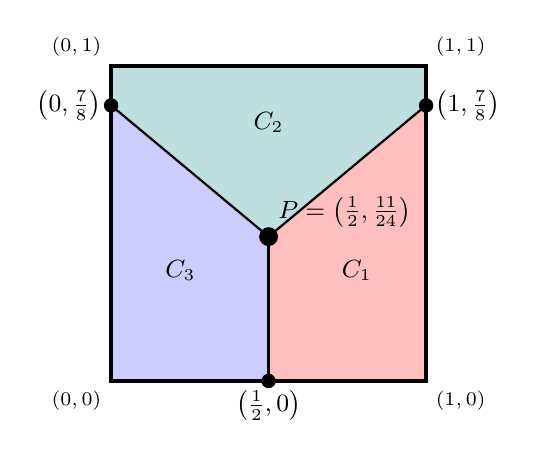
\begin{tikzpicture}[scale=4]
  % Square
  \draw[thick] (0,0) rectangle (1,1);

  % Pieces (filled)
  \fill[red!25] (0.5,0.4583) -- (0.5,0) -- (1,0) -- (1,0.875) -- cycle;
  \fill[teal!25] (0.5,0.4583) -- (1,0.875) -- (1,1) -- (0,1) -- (0,0.875) -- cycle;
  \fill[blue!20] (0.5,0.4583) -- (0,0.875) -- (0,0) -- (0.5,0) -- cycle;

  % Cuts
  \draw[thick] (0.5, 0.4583) -- (0.5, 0);
  \draw[thick] (0.5, 0.4583) -- (1, 0.875);
  \draw[thick] (0.5, 0.4583) -- (0, 0.875);

  % Square border (redraw on top)
  \draw[very thick] (0,0) rectangle (1,1);

  % Points
  \filldraw (0.5, 0.4583) circle (0.8pt) node[above right, font=\small]
    {$P = \bigl(\frac{1}{2},\frac{11}{24}\bigr)$};
  \filldraw (0.5, 0) circle (0.6pt)
    node[below, font=\small] {$\bigl(\frac{1}{2}, 0\bigr)$};
  \filldraw (1, 0.875) circle (0.6pt)
    node[right, font=\small] {$\bigl(1, \frac{7}{8}\bigr)$};
  \filldraw (0, 0.875) circle (0.6pt)
    node[left, font=\small] {$\bigl(0, \frac{7}{8}\bigr)$};

  % Labels
  \node[font=\small\bfseries] at (0.78, 0.35) {$C_1$};
  \node[font=\small\bfseries] at (0.5, 0.82) {$C_2$};
  \node[font=\small\bfseries] at (0.22, 0.35) {$C_3$};

  % Corner labels
  \node[below left, font=\scriptsize] at (0,0) {$(0,0)$};
  \node[below right, font=\scriptsize] at (1,0) {$(1,0)$};
  \node[above right, font=\scriptsize] at (1,1) {$(1,1)$};
  \node[above left, font=\scriptsize] at (0,1) {$(0,1)$};
\end{tikzpicture}
\end{center}

\begin{itemize}
\item Interior point: $P = \bigl(\tfrac{1}{2}, \tfrac{11}{24}\bigr)$.
\item Three cuts to boundary points:
  $\bigl(\tfrac{1}{2}, 0\bigr)$,
  $\bigl(1, \tfrac{7}{8}\bigr)$,
  $\bigl(0, \tfrac{7}{8}\bigr)$.
\end{itemize}

\medskip
The three pieces are:

\begin{align*}
  C_1 &= \operatorname{conv}\!\Bigl\{
    \bigl(\tfrac{1}{2}, \tfrac{11}{24}\bigr),\;
    \bigl(\tfrac{1}{2}, 0\bigr),\;
    (1, 0),\;
    \bigl(1, \tfrac{7}{8}\bigr)
  \Bigr\},\\[4pt]
  C_2 &= \operatorname{conv}\!\Bigl\{
    \bigl(\tfrac{1}{2}, \tfrac{11}{24}\bigr),\;
    \bigl(1, \tfrac{7}{8}\bigr),\;
    (1,1),\; (0,1),\;
    \bigl(0, \tfrac{7}{8}\bigr)
  \Bigr\},\\[4pt]
  C_3 &= \operatorname{conv}\!\Bigl\{
    \bigl(\tfrac{1}{2}, \tfrac{11}{24}\bigr),\;
    \bigl(0, \tfrac{7}{8}\bigr),\;
    (0,0),\;
    \bigl(\tfrac{1}{2}, 0\bigr)
  \Bigr\}.
\end{align*}

\subsection{Verification of equal areas}

Using the shoelace formula, we verify each area exactly:

\paragraph{Piece $C_1$ (right quadrilateral).}
Vertices in order:
$\bigl(\tfrac{1}{2},\tfrac{11}{24}\bigr)$,
$\bigl(\tfrac{1}{2},0\bigr)$,
$(1,0)$,
$\bigl(1,\tfrac{7}{8}\bigr)$.
\[
  \operatorname{Area}(C_1) = \tfrac{1}{2}\bigl|
    \tfrac{1}{2}\cdot 0 - \tfrac{1}{2}\cdot\tfrac{11}{24}
    + \tfrac{1}{2}\cdot 0 - 1\cdot 0
    + 1\cdot\tfrac{7}{8} - 1\cdot 0
    + 1\cdot\tfrac{11}{24} - \tfrac{1}{2}\cdot\tfrac{7}{8}
  \bigr|
  = \frac{1}{3}.
\]

\paragraph{Piece $C_3$ (left quadrilateral).}
By the reflection $x \mapsto 1-x$, this is congruent to $C_1$, so
$\operatorname{Area}(C_3) = \tfrac{1}{3}$.

\paragraph{Piece $C_2$ (top pentagon).}
$\operatorname{Area}(C_2) = 1 - \tfrac{1}{3} - \tfrac{1}{3} = \tfrac{1}{3}$.

\subsection{Diameter computation}

\begin{theorem}
All three pieces have diameter exactly
\[
  d^* = \sqrt{\frac{65}{64}} = \frac{\sqrt{65}}{8} \approx 1.00778.
\]
\end{theorem}

\begin{proof}
For each piece, we compute the maximum pairwise distance among its
vertices (which equals the diameter for convex polygons).

\paragraph{Piece $C_1$.}
The six pairwise distances squared are:
\begin{center}
\begin{tabular}{lll}
\toprule
Pair & $d^2$ & Value \\
\midrule
$\bigl(\frac{1}{2},\frac{11}{24}\bigr) \leftrightarrow \bigl(\frac{1}{2},0\bigr)$
  & $\bigl(\frac{11}{24}\bigr)^2 = \frac{121}{576}$ & $0.2100$ \\[3pt]
$\bigl(\frac{1}{2},\frac{11}{24}\bigr) \leftrightarrow (1,0)$
  & $\frac{1}{4} + \frac{121}{576} = \frac{265}{576}$ & $0.4601$ \\[3pt]
$\bigl(\frac{1}{2},\frac{11}{24}\bigr) \leftrightarrow \bigl(1,\frac{7}{8}\bigr)$
  & $\frac{1}{4} + \bigl(\frac{7}{8}-\frac{11}{24}\bigr)^2 = \frac{61}{144}$ & $0.4236$ \\[3pt]
$\bigl(\frac{1}{2},0\bigr) \leftrightarrow (1,0)$
  & $\frac{1}{4}$ & $0.2500$ \\[3pt]
$\bigl(\frac{1}{2},0\bigr) \leftrightarrow \bigl(1,\frac{7}{8}\bigr)$
  & $\frac{1}{4} + \frac{49}{64} = \mathbf{\frac{65}{64}}$ & $\mathbf{1.0156}$ \\[3pt]
$(1,0) \leftrightarrow \bigl(1,\frac{7}{8}\bigr)$
  & $\frac{49}{64}$ & $0.7656$ \\
\bottomrule
\end{tabular}
\end{center}
The maximum is $\frac{65}{64}$, achieved by the pair
$\bigl(\frac{1}{2},0\bigr) \leftrightarrow \bigl(1,\frac{7}{8}\bigr)$,
giving $\operatorname{diam}(C_1) = \sqrt{65}/8$.

\paragraph{Piece $C_3$.}
By reflection symmetry, $\operatorname{diam}(C_3) = \sqrt{65}/8$.

\paragraph{Piece $C_2$.}
The diametrically opposite pairs are
$\bigl(1,\tfrac{7}{8}\bigr) \leftrightarrow (0,1)$ and
$\bigl(0,\tfrac{7}{8}\bigr) \leftrightarrow (1,1)$, both with
\[
  d^2 = 1^2 + \bigl(1 - \tfrac{7}{8}\bigr)^2 = 1 + \tfrac{1}{64} = \frac{65}{64}.
\]
All other pairs yield strictly smaller distances (verified
computationally). Thus $\operatorname{diam}(C_2) = \sqrt{65}/8$.
\end{proof}

%% ─────────────────────────────────────────────────────
\section{Why Does the Y-Partition Beat Strips?}

The key geometric insight is that the strip partition forces each piece
to span the \emph{full width} of the square. The diameter of a
$\tfrac{1}{3}\times 1$ rectangle is dominated by its long diagonal.

The Y-partition avoids this: no single piece spans the full width
\emph{and} the full height. Instead, the three cuts from the interior
point create compact pieces whose diameters are governed by
``cross-diagonal'' distances that are shorter than $\sqrt{1^2 +
(\frac{1}{3})^2}$.

Quantitatively:
\[
  \frac{\sqrt{65}/8}{\sqrt{10}/3}
  = \frac{3\sqrt{65}}{8\sqrt{10}}
  = \frac{3\sqrt{65}}{8\sqrt{10}} \approx 0.956,
\]
a $4.4\%$ reduction.

%% ─────────────────────────────────────────────────────
\section{Comparison of Topologies}

\begin{center}
\renewcommand{\arraystretch}{1.3}
\begin{tabular}{lccc}
\toprule
\textbf{Topology} & \textbf{Max diameter} & \textbf{Exact} & \textbf{vs.\ strips} \\
\midrule
Y-partition (optimal) & $1.00778$ & $\sqrt{65}/8$ & --- \\
Parallel strips & $1.05409$ & $\sqrt{10}/3$ & $+4.6\%$ \\
T-partition & $1.05409$ & $\sqrt{10}/3$ & $+4.6\%$ \\
Y from center to corners & $1.11803$ & $\sqrt{5}/2$ & $+10.9\%$ \\
Fan partition & $1.11803$ & $\sqrt{5}/2$ & $+10.9\%$ \\
Adjacent corner cuts & $1.23024$ & --- & $+22.1\%$ \\
\bottomrule
\end{tabular}
\end{center}

%% ─────────────────────────────────────────────────────
\section{Computational Methodology}

The optimization was performed in Python using SciPy's
\texttt{differential\_evolution} global optimizer:

\begin{enumerate}
\item \textbf{Topology enumeration.}
  Three partition families were implemented: nested chords, adjacent
  chords, and Y-partitions.

\item \textbf{Boundary parameterization.}
  Boundary points of the unit square were parameterized by a single
  perimeter coordinate $t \in [0,4)$, mapping counterclockwise from the
  origin.

\item \textbf{Objective function.}
  $\max_i \operatorname{diam}(C_i)$ with a quadratic penalty for
  area deviation from $\tfrac{1}{3}$.

\item \textbf{Symmetry exploitation.}
  The Y-partition was refined using a 2-parameter symmetric
  formulation ($p_y$ and $a$), enabling a fine grid search and
  high-precision optimization ($\texttt{tol} = 10^{-15}$).

\item \textbf{Exact recovery.}
  The numerical solution $(p_y \approx 0.458333,\; a \approx 0.875)$
  was identified as $p_y = \tfrac{11}{24}$, $a = \tfrac{7}{8}$.
  All areas and diameters were then verified using exact rational
  arithmetic.
\end{enumerate}

%% ─────────────────────────────────────────────────────
\section{Open Questions}

\begin{enumerate}
\item \textbf{Global optimality.}
  Is $\sqrt{65}/8$ the true global minimum across \emph{all} possible
  topologies? Our search covered the three main combinatorial families,
  but a rigorous lower-bound argument (e.g.\ via the isodiametric
  inequality combined with tiling constraints) would be needed for a
  complete proof.

\item \textbf{Lower bound.}
  The isodiametric inequality gives $d \geq 2\sqrt{1/(3\pi)} \approx
  0.651$ for any convex piece of area $\tfrac{1}{3}$. The gap between
  this and $\sqrt{65}/8 \approx 1.008$ suggests room for a tighter
  bound that accounts for the tiling constraint.

\item \textbf{Generalization to $n$ pieces.}
  What is the optimal partition of a square into $n$ equal-area convex
  pieces for general $n$? The answer is known for $n = 2$ (two
  rectangles) and $n = 4$ (four squares), but the intermediate cases
  remain open.
\end{enumerate}

\end{document}
